\documentclass[12pt]{article}
\usepackage{minted}
\usepackage[pdftex]{graphicx}
\usemintedstyle{emacs}

%opening
\title{Assignment \#2\\Discovering Affixes Automatically}
\author{Thuong-Hai Pham}

\begin{document}

\maketitle

\begin{abstract}

\end{abstract}

\section{TrieNode} \label{trienode}

\subsection{Fields}
\begin{center}
	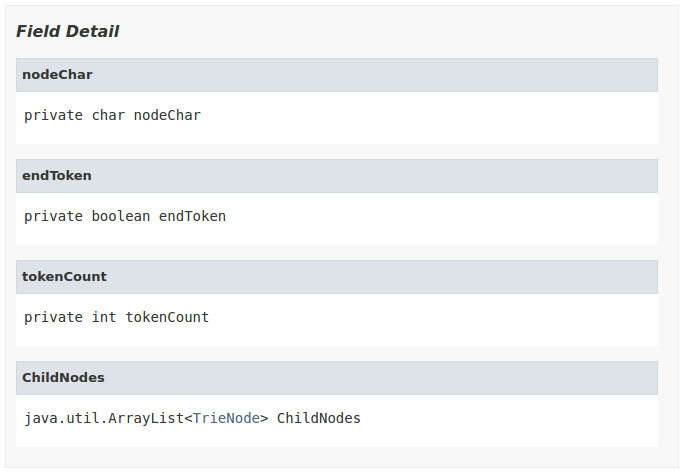
\includegraphics[width=\textwidth]{trie_node_fields}
\end{center}

% Requirement: In your documentation take care to explain clearly why only one node class is required, and demonstrate how you cater for the different node ‘types’ with one class.
Although we have three different kinds of node in our algorithm, these nodes are implemented in only one single class because the attributes in this class and the way we construct our algorithm help distinguishing an instance into these three kinds.

First, every node instance is created (equal and) to be ``regular node". Then, by having the attribute ``endToken" set to true or false, it will be considered as ``end token node" or still ``regular node", respectively.

After introducing ``endToken" attribute, the only problem is how to mark ``root node" from those two. If we look closely to the diagram, there is only one root node which has no parent, i.e. no node points to this root node as its child. Hence, we will have to handle this node from outside the tree, e.g. in ``main class" or in 
``Trie Dictionary" (which will be implemented later). Therefore, there is no need to mark one node is root or not.

\subsection{Methods}
% Next item to consider: each node can have several children. How would you store these children? Remember, these are nodes as well. So in your node class, you need storage for a list of children of type Node.
Our straightforward approach to manage the child nodes is to create an ArrayList (supported by Java) of TrieNode to handle child nodes of a specific node.
\begin{listing}[ht]
	\begin{minted}[frame=single]{java}
	ArrayList<TrieNode> ChildNodes = new ArrayList<>();
	\end{minted}
	\caption{Declaration of ChildNodes}
\end{listing}

Whenever we need to add a new child node (e.g. add new entry), we first check whether it exists then initiate the new one, add it in the list.


\begin{listing}[ht]
	\begin{minted}[frame=single]{java}
	TrieNode t = this.getChildNode(input.charAt(0));
	if (t == null) {
		t = new TrieNode(input.charAt(0));
		this.ChildNodes.add(t);
	}
	\end{minted}
	\caption{Add new child node}
\end{listing}

\begin{center}
	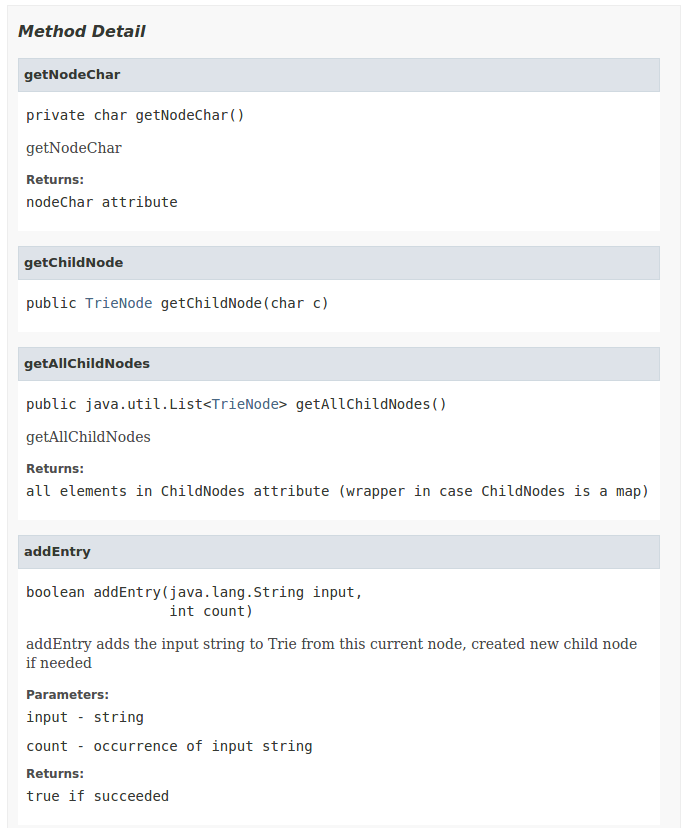
\includegraphics[width=\textwidth]{trie_node_methods}
\end{center}
\begin{center}
	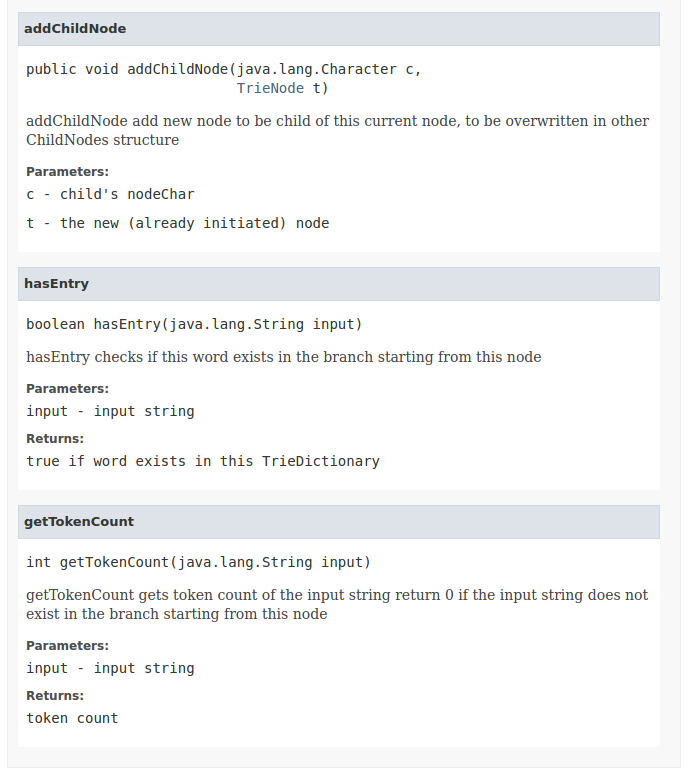
\includegraphics[width=\textwidth]{trie_node_methods_b}
\end{center}

\section{TrieNodeAdv} \label{trienodeadv}

However, the simple and straightforward approach above may face a disadvantage in which our algorithm has to search throughout all of elements of ChildNodes to find out the queried child. Hence, we implemented an advanced version of our TrieNode by inheriting TrieNode with modification of its ChildNodes attribute.

In this version, ChildNodes is implemented with a Java HashMap. This data structure helps to reduce the complexity of child searching from O(n) (n is number of elements in ChildNodes) down to approximation of O(logn) by searching and hash function.

\begin{center}
	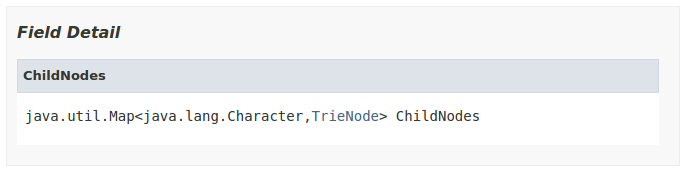
\includegraphics[width=\textwidth]{trie_node_adv_fields}
\end{center}

\section{Trie Dictionary}

Our TrieDictionary serves as a wrapper or entry point for the whole Trie itself, which basically holds the root node as mentioned in section \ref{trienode}.

\subsection{Fields}
\begin{center}
	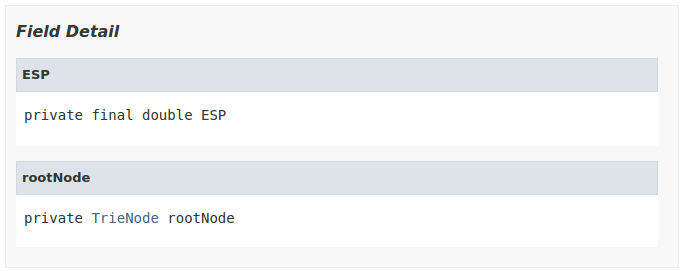
\includegraphics[width=\textwidth]{trie_dictionary_fields}
\end{center}

\subsection{Methods}
\begin{center}
	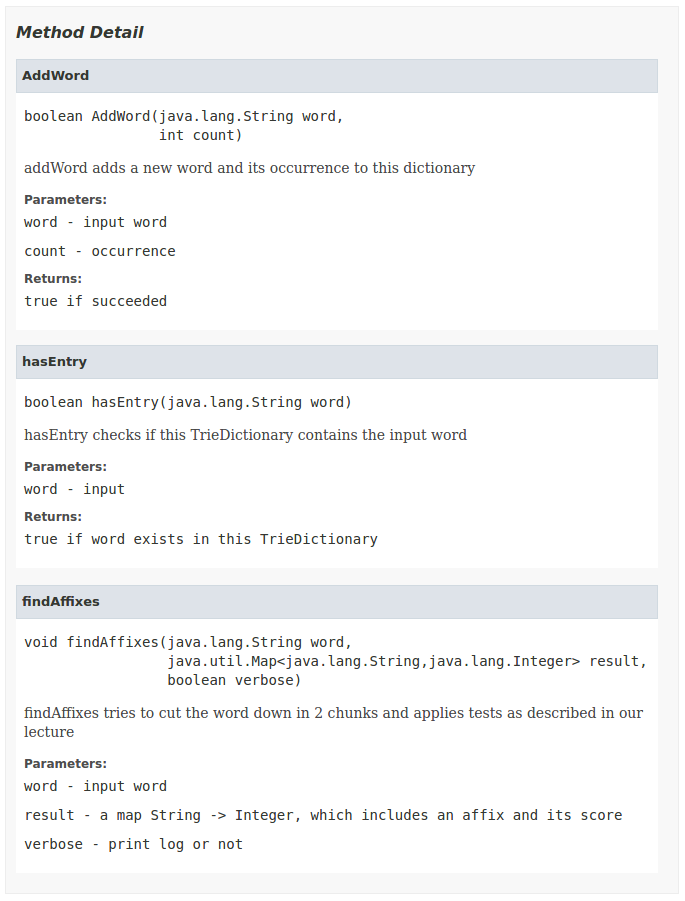
\includegraphics[width=\textwidth]{trie_dictionary_methods}
\end{center}

\begin{center}
	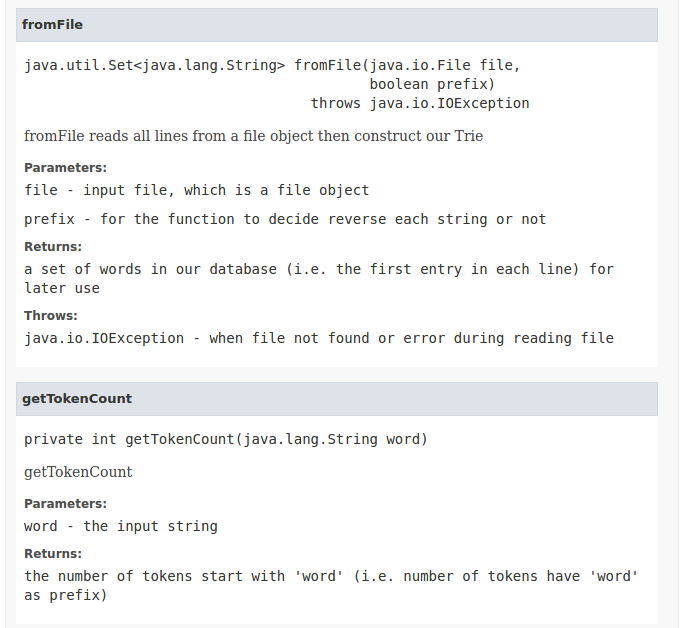
\includegraphics[width=\textwidth]{trie_dictionary_methods_b}
\end{center}

In this class, we also implemented the affixes finding method to discover affixes in the whole Trie by examining the three criteria.

This also justifies the need of constant variable ESP (epsilon) which helps us to do the approximate comparison of ``approximate to 1" and ``much less than 1". 


\begin{listing}[H]
	\begin{minted}[frame=single]{java}
void findAffixes(String word, Map<String, Integer> result,
	boolean verbose) {
	...
	boolean test1 = this.hasEntry(alphaA);
	boolean test2 = Math.abs((float) freqAlphaA / 
	freqAlpha - 1) < ESP;
	boolean test3 = (float) freqAlphaAB / 
	freqAlphaA < 1 - ESP;
	...
}
	\end{minted}
	\caption{Affixes criteria}
\end{listing}

\section{Main Class}


Main class is home for our program entry point, and also equipped with a utility string reversing function. In Main, we also implemented a test as described in our assignment instruction to make sure the implementation basic functions work well before running with large datasets.

\begin{center}
	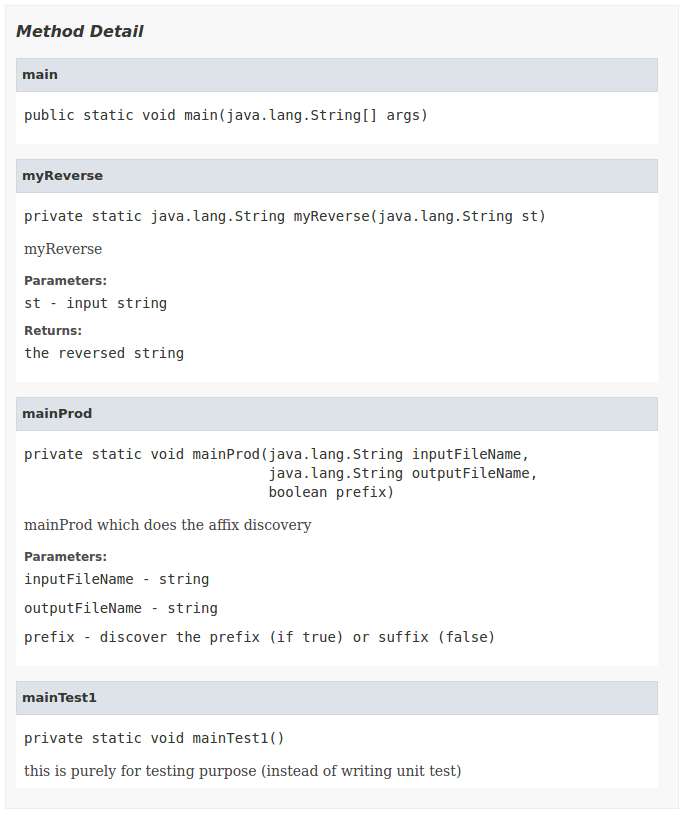
\includegraphics[width=\textwidth]{main_methods}
\end{center}

\section{Research question}
\subsection{Computational perspective}

As discussed in section \ref{trienodeadv}, TrieNodeAdv is implemented with HashMap from Java in an attempt to prevent linear search throughout ChildNodes and to reduce our complexity for that part from O(n) to O(logn). By running those two on our real dataset English.txt, we get the following result. (running time is measured in second (S))

\begin{listing}[H]
	\begin{minted}[frame=single]{text}
TrieNode
	Constructing tree from file: PT4.978S
	Discovering affixes: PT10.413S

TrieNodeAdv
	Constructing tree from file: PT4.495S
	Discovering affixes: PT10.007S
	\end{minted}
	\caption{Speed testing output TrieNode and TrieNodeAdv}
\end{listing}

It is clear that TrieNodeAdv is faster than its parent class. However, this improvement is subtle due to one possible explanation. The number of child nodes is varied, and does not always reach the limit of around 30. Therefore, the real n in average is much less than 30, which does not leverage O(n)-to-O(logn) improvement.

\subsection{Linguistic perspective}
As we can see in the output files, the algorithm worked pretty well when having discovered these top (sorted by scores) prefixes and suffixes:
\begin{table}[H]
	\begin{tabular}{| p{6.5cm} | p{6.5cm} |}
		\hline
		Prefixes & Suffixes \\
		\hline
		un 48609\newline
		re 27857\newline
		non 12638\newline
		in 12162\newline
		dis 11215\newline
		sub 11149\newline
		de 10921\newline
		bio 8965\newline
		micro 8893\newline
		get 8750\newline
		pre 8367\newline
		over 7909
		& 
		s 521319\newline
		ly 60223\newline
		ing 43367\newline
		ed 41247\newline
		ness 19834\newline
		ers 15311\newline
		es 13903\newline
		ism 12712\newline
		ally 12689\newline
		al 10715\newline
		ist 8997\newline
		er 7911\\
		\hline
	\end{tabular}
\end{table}
However, there exists an issue in which ``-ers" shows up among its building-block real suffixes ``-er" and ``-s". This problem can be solved by prunning \cite{keshava2006simpler}, in which we scan through our affixes list again. While scanning, if there exists a morpheme that is a concatenation of other two morphemes with higher scores, the unfortunate morpheme should be removed from our list.

One more problem in our algorithm is that some affixes are penalised so badly that they can not make themself to the final list. For example, the suffix of ``-en" in ``lengthen 1007", ``strengthen 23200", ``shorten 2621", ``harden 1822" should be listed, yet not because it is penalised by its existence in ``heaven 47060", ``garden 176285" and similar nouns. It is obvious that this issue and its similar situations can be solved by distinguishing the Part-of-speech (POS) of both words and their segmented morphemes.

In the two problems above, solution for the first one still keeps the unsupervised nature of our algorithm. On the other hand, the second one, which requires an additional information, turns our algorithm into semi-supervised.

\bibliographystyle{apalike}
\bibliography{trie-report}

\end{document}
